\subsection{Experimental Results addressing Research Questions (RQ1-3):}
\label{subsec:experimental_results}

\begin{figure}[ht]
  \centering
  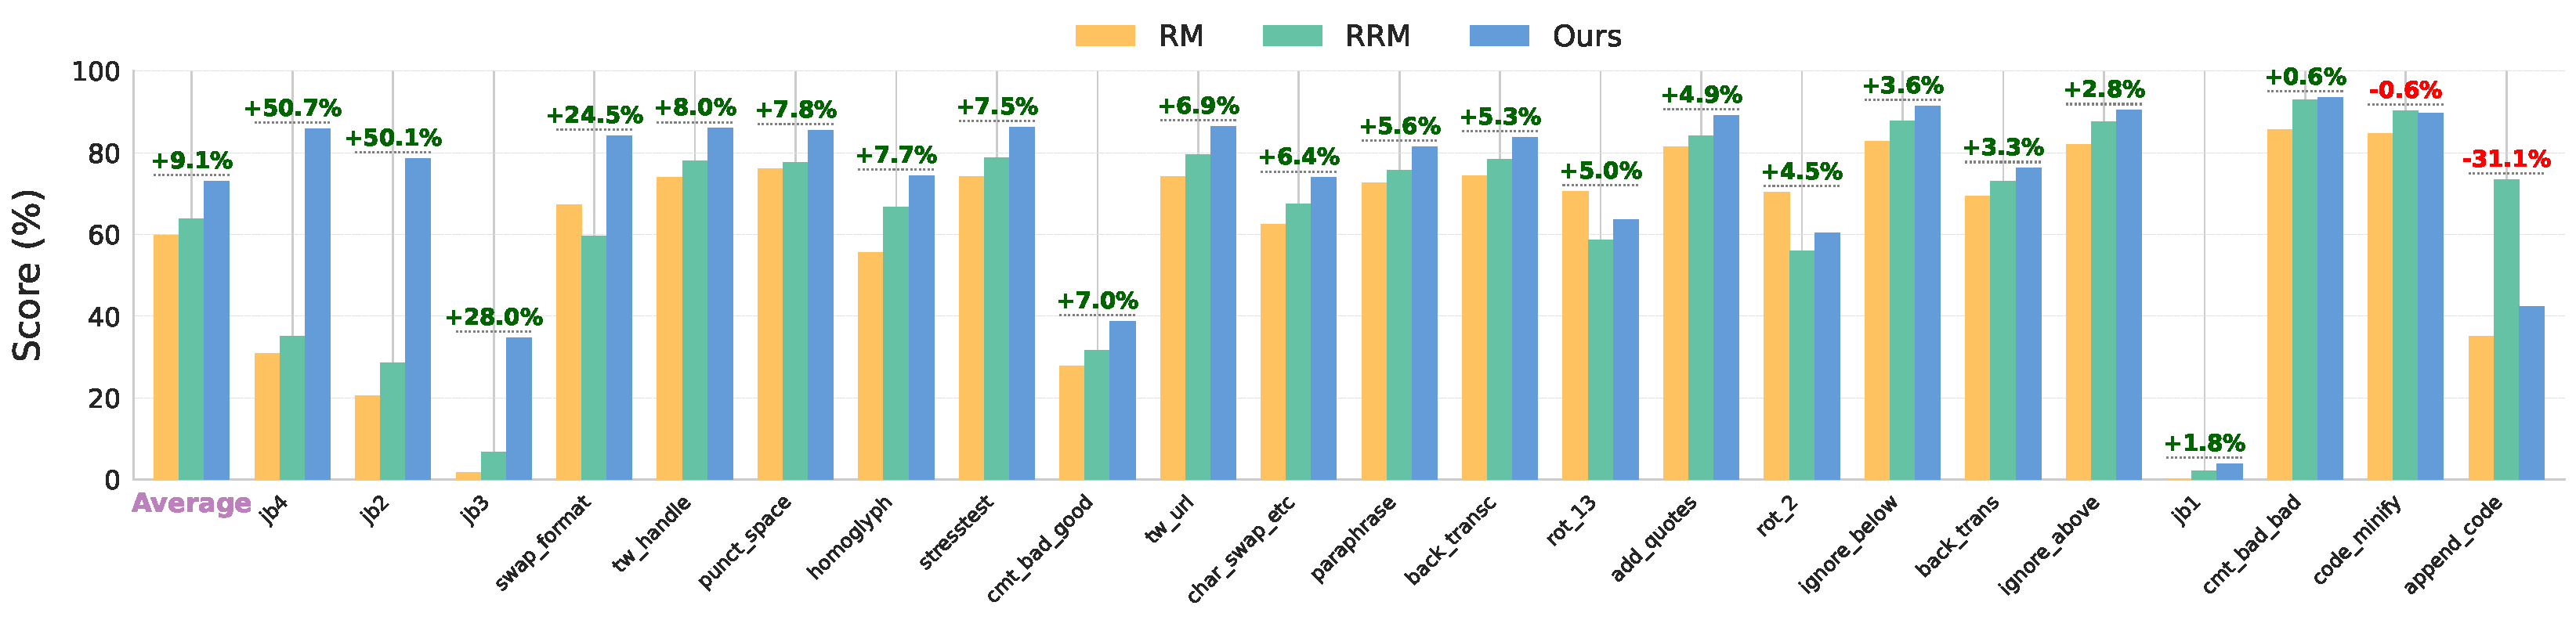
\includegraphics[width=1.0\columnwidth]{images/reword_absolute_robustness_gemma9b_pairpm_sorted.pdf}
  \caption{\textbf{Robustness of \carma{}} on reWordBench. Comparing RM, RRM and \carma{} by measuring ranking accuracy on a diverse set of meaning preserving transformations in reWordBench. Various transformations such as paraphrasing, addition of irrelevant text or code, comments etc, test the sensitivity of models to spuriousness. Robust training of \carma{} leads to robustness to spuriousness and increased sensitivity to causal attributes.
  }
  \label{fig:reword_absolute_robustness_gemma9b_pairpm}
\vspace{0.2in}  
\end{figure}

On \textbf{RewardBench} (Table~\ref{tab:performance_bt_pairpm_rewardbench_extended_final}), \carma{} consistently improves ranking accuracy over RRM across diverse base models and reward modeling techniques (PairPM, BT).
These improvements are particularly notable on the challenging \textit{Safety} (up to \changeUp{13.18\%}) and \textit{Reasoning} (up to \changeUp{7.19\%}). \carma{} also demonstrates superior robustness on \textbf{reWordBench}, which tests for robustness of RMs against meaning-preserving transformations (Figure~\ref{fig:reword_absolute_robustness_gemma9b_pairpm}). 

These results show \carma{}'s robustness to inputs having spurious punctations, paraphrasing, irrelevant text, code or comments as tested by various reWordBench transformations. With \gemmait{9}, \carma{} in the PairPM setting shows an aggregate accuracy gain of up to \changeUp{9.1\%} and is superior on \textcolor{PaperGreen}{(21/23)} transformations.

\vspace{0.25in}
\begin{takeawaybox}
\textbf{Key Takeaway:} \carma{} improves RM performance on standard benchmarks while significantly improving performance and mitigating ranking accuracy drops on diverse transformed inputs, \textit{without ever being explicitly trained on such spurious transformations}.
\end{takeawaybox}
\vspace{0.1in}

\clearpage
% \vspace{0.1in}
\paragraph{BoN for Robust LLM Alignment Across Chat, Reasoning, and Safety} Following the method used by \citet{wu2025rewordbench}, we perform best-of-n selection using \carma\ across RewardBench categories, which consists of datasets such as AlpacaEval. Across all values of $N$, \carma\ provided significant improvements over baselines in a head-to-head comparison.

\vspace{0.05in}
\begin{takeawaybox}
\textbf{Key Takeaway:} \carma's emphasis on causal attributes enhances its discriminative power in Best-of-N selection, leading to more consistent identification of superior responses.
\end{takeawaybox}
\vspace{0.05in}

\begin{table}[ht]
    \centering
    \resizebox{0.58\linewidth}{!}{%
    \begin{tabular}{@{} c
            S[table-format=2.2] S[table-format=2.2] S[table-format=2.2]
            S[table-format=2.2] S[table-format=2.2] S[table-format=2.2] @{}}
            \toprule
            \multirow{2}{*}{\textbf{N}} &
            \multicolumn{3}{c}{\textbf{\carma{} vs RM}} &
            \multicolumn{3}{c}{\textbf{\carma{} vs RRM}} \\
            \cmidrule(lr){2-4}\cmidrule(lr){5-7}
            & {\carma{}} & {RM} & {Ties} & {\carma{}} & {RRM} & {Ties} \\
            \midrule
            4  & \textbf{28.08} & 13.85 & 58.07 & \textbf{28.03} & 14.13 & 57.84 \\
            8  & \textbf{34.32} & 17.24 & 48.43 & \textbf{34.36} & 17.19 & 48.45 \\
            16 & \textbf{39.93} & 20.54 & 39.53 & \textbf{41.14} & 20.40 & 38.46 \\
            32 & \textbf{44.79} & 21.88 & 33.33 & \textbf{45.46} & 22.01 & 32.53 \\
            \bottomrule
    
    \end{tabular}
    }
    \caption{\textbf{Win rates for \carma{} compared with RM and RRM on RewardBench}. We follow \citet{wu2025rewordbench} and take all 2985 prompts from RewardBench and get BoN responses from a \gemmait{9} model using \carma{}, RM or RRM as the reward models. Following this, we separately compare responses generated by \carma{} with RM and RRM, using GPT-4 as a judge.\vspace{-0.1in}}
    \label{tab:bon_results_rewardbench}
\end{table}

\begin{figure}[ht]
    \centering
    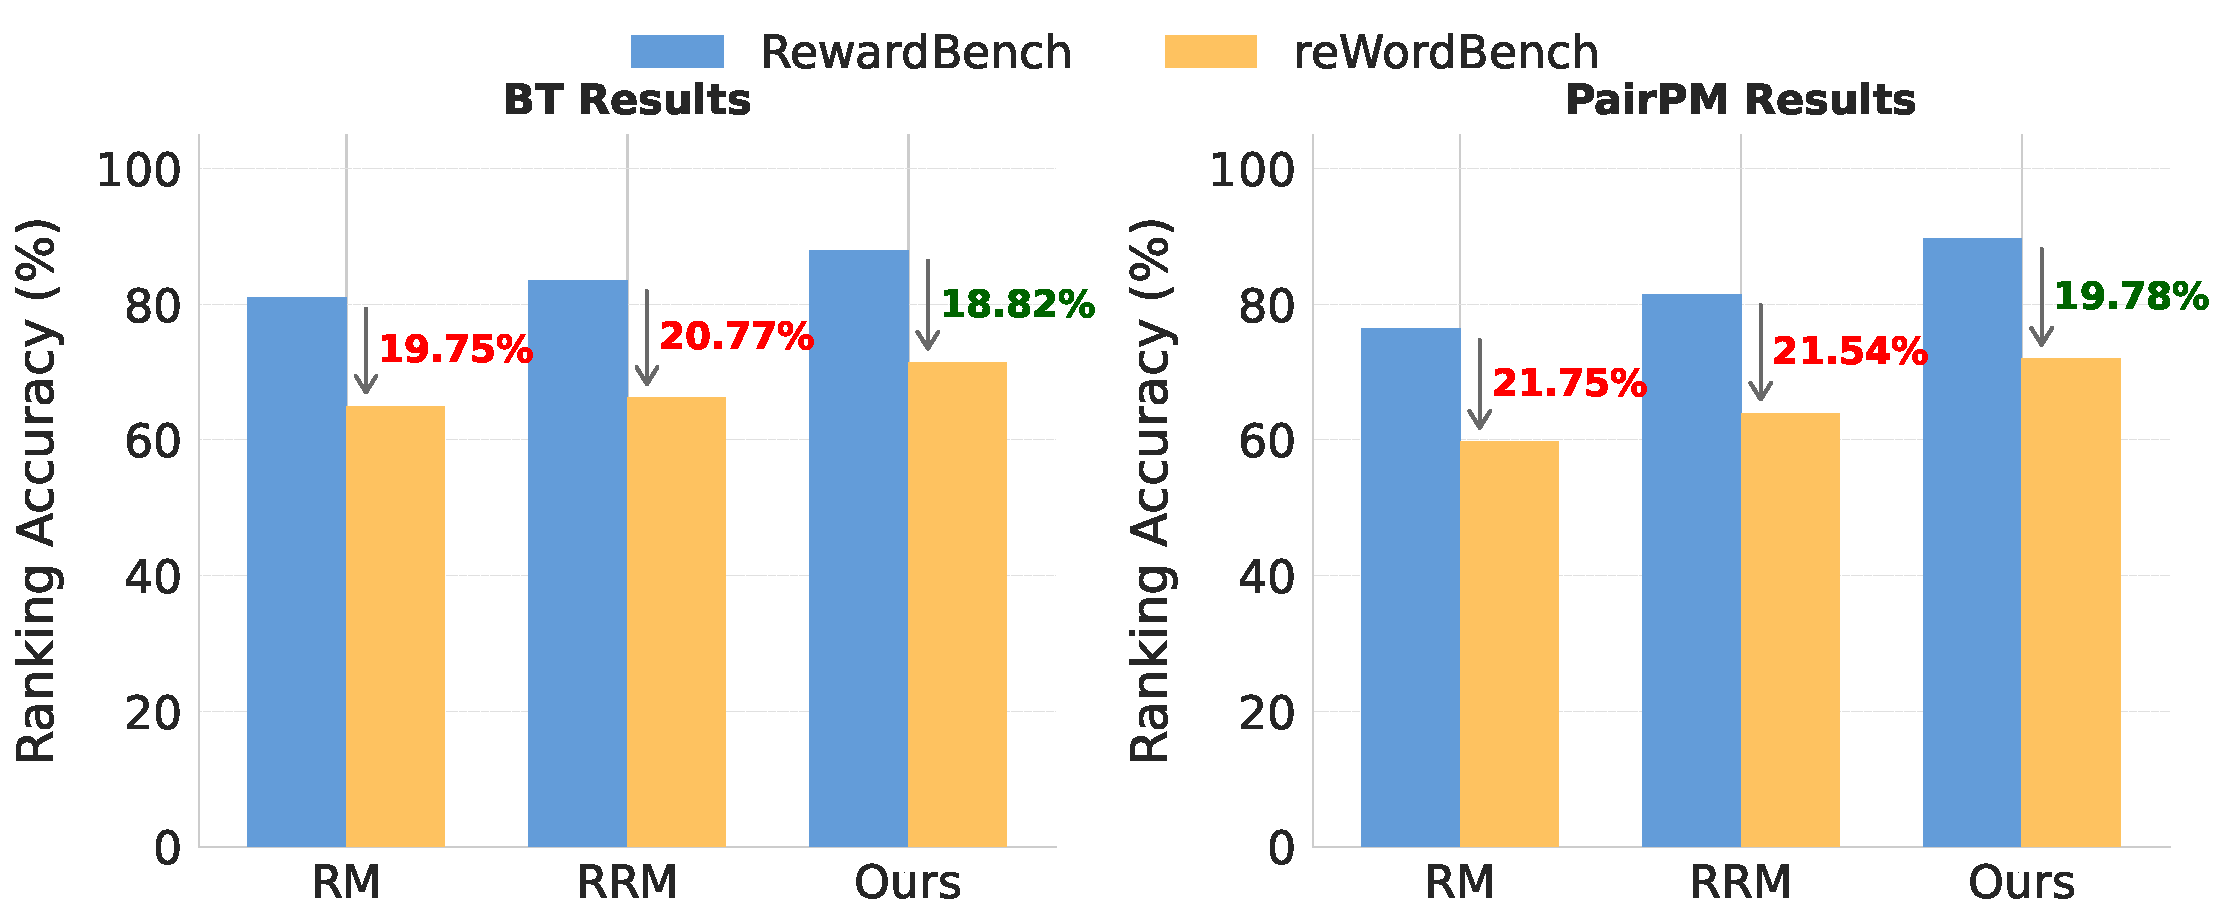
\includegraphics[width=0.7\linewidth]{images/reword_ranking_acc_drop_gemma9b_bt_pairpm_blueyellow.pdf}
    \caption{\textbf{Percentage improvement in ranking accuracy} between RewardBench and reWordBench. Here we show the average ranking accuracy across reWordBench transformations of \carma{} and baselines on reWordBench and RewardBench as done in \citet{wu2025rewordbench}, as well as the percentage drop in ranking accuracy on reWordBench compared to RewardBench. We show that \carma{}'s ranking accuracy percentage drop going from RewardBench to reWordBench is the lowest compared to baselines.\vspace{-0.1in}}
    \label{fig:reword_ranking_acc_drop_gemma9b_bt_pairpm}
\end{figure}

\paragraph{Ranking Accuracy Percentage Improvements:}
We measure the percentage drop in response ranking accuracy between RewardBench and reWordBench scores (following the macro-avg metric used in \citet{wu2025rewordbench}). \carma{} exhibits a smaller ranking accuracy percentage drop from RewardBench to reWordBench (In case of PairPM: $19.78$\% vs. RRM's $21.54$\%. See  Figure \ref{fig:reword_ranking_acc_drop_gemma9b_bt_pairpm} for the results on BT and PairPM settings.

\vspace{0.02in}
\begin{takeawaybox}
\textbf{Key Takeaway:} Assuming sufficient concentration of spurious elements in the prompt as well as the $N$ responses, \carma{} is better at selecting the best response based on causal attributes only. For e.g., in safety, harmful prompts and responses may be spuriously disguised as benign. 
\end{takeawaybox}

\clearpage

\begin{figure}[!h]
  \centering
  \begin{minipage}[t]{0.45\textwidth}
  % \vspace{-0.1in}
  \paragraph{Causal Attributes help in detecting jailbreaks}
For \gemmait{9} as the solution generation model, BoN with \carma{} shows significant improvements on safety as measured on WildGuardTest. In particular the attack success ratio (ASR) on harmful prompts is much lower compared to models aligned with RM and RRM and this gap increases with N. This improved ASR comes at at a similar refusal-to-answer rate on benign prompts.

  \end{minipage}\hfill          % \hfill inserts a flexible gutter
  \begin{minipage}[t]{0.50\textwidth}
    \vspace{-0.15in}
    \centering
    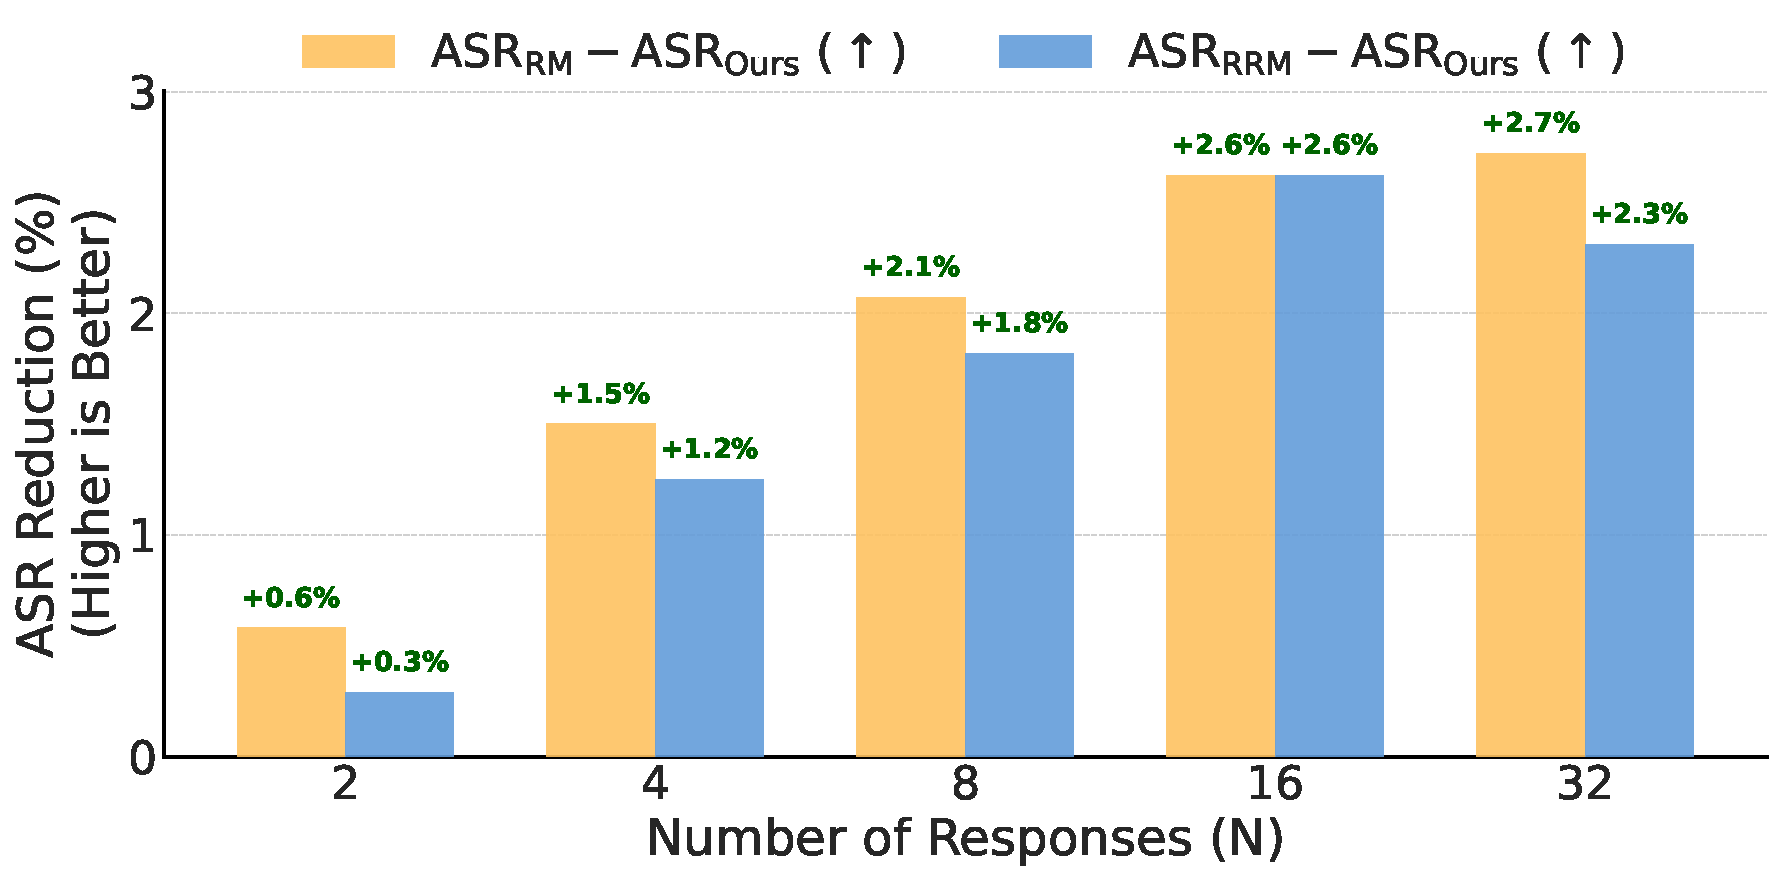
\includegraphics[width=0.95\linewidth]{images/asr_reduction_gemma9B_pairpm.pdf}
    \vspace{-0.10in}
    \captionof{figure}{Best-of-N results: ASR reduction on WildGuardTest. }
    \label{fig:asr_reduction_gemma9b}
  \end{minipage}


\vspace{0.03in}
\begin{takeawaybox}
\textbf{Key Takeaway:} \carma{}'s causal augmentations achieve a superior trade-off between safety and over-refusals, because its contrastive pairs delineate the decision boundary for harmful content more faithfully. This leads to safer content, while avoiding excessive refusals on benign prompts.

\end{takeawaybox}
\vspace{0.03in}
\end{figure}

\vspace{0.03in}
\begin{figure}[!ht]
  \centering
  \begin{minipage}[t]{0.48\textwidth}
  \vspace{0.0in}
    \centering
    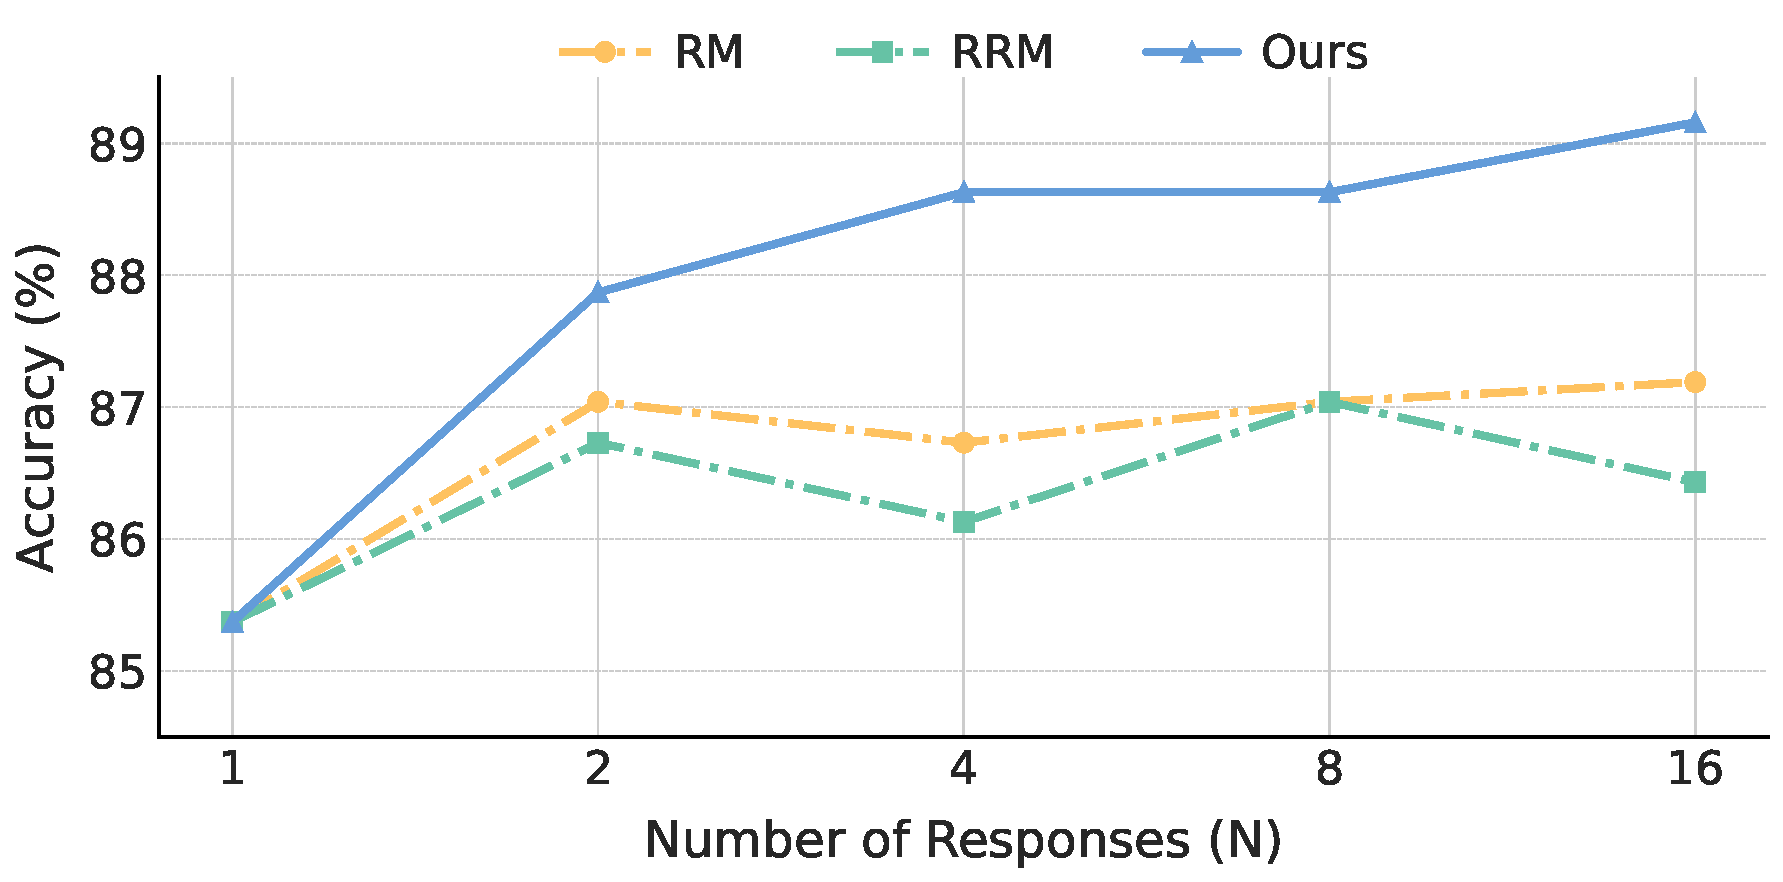
\includegraphics[width=0.9\linewidth]{images/bon_gsm8k_gemma9b_pairpm.pdf}
    % \vspace{-0.10in}
    \captionof{figure}{Best-of-N Reasoning evaluation on GSM8K.}
    \label{fig:bon_gsm8k_gemma9b}
  \end{minipage}\hfill          % \hfill inserts a flexible gutter
  \begin{minipage}[t]{0.48\textwidth}
  \vspace{0.0in}
  \paragraph{Disentangling Content related features from stylistic (spurious) ones helps in reasoning}

For \gemmait{9} as the solution generation model on GSM8K, \carma{} shows a consistent gap over baseslines across different values of $N$.
Non robust reward models may focus on stylistic details. Good looking, detailed but wrong reasoning steps may mis-guide non-robust RMs into giving a higher score to the response.
\end{minipage}

\vspace{0.03in}
\begin{takeawaybox}
\textbf{Key Takeaway:} Reasoning correctness is dependent on focusing on correctness over stylistic features. Our training ensures \carma{} is good at capturing content-features over other attributes. 
\end{takeawaybox}
\vspace{0.03in}
\end{figure}


\vspace{-0.22in}
\subsection{Neutral Ablations}
\label{ssec:neutral_ablations}

\vspace{-0.1in}
Along with IQN, we tested several methods for enforcing spurious invariance:

\vspace{-0.15in}
\paragraph{Causally Aligned Neutrals (CAN).} 
Given a preference pair $(A_w, A_\ell)$ where $(A_w \succ A_\ell)$, 
we rewrite $A_\ell$ into $\tilde{A}_\ell$ such that the causal content of $\tilde{A}_\ell$ aligns with $A_w$ ($C(A_w) \approx C(\tilde{A}_l)$), but due to the rewrite from $A_\ell$, the spurious attributes of $A_\ell$ remain. By assigning a tie-label to this pair during training, we force the model to learn invariance to the spurious differences. While this method is sound theoretically, the approximation of $C(A_w)$ by $C(\tilde{A}_l)$ is not perfect. Furthermore, some spurious attributes $SP'(\tilde{A}_l) \subset SP(\tilde{A}_l)$ vary when we move causal attributes. Invariance to these attributes $SP'(\tilde{A}_l)$ is not captured by CAN.


\vspace{-0.15in}
\paragraph{Paraphrase Neutral (PARA).} Given an answer $A$ to a query $Q$, we rewrite $A$ to an approximate $\tilde{A}$ using an LLM, such that spurious features vary, but causal features do not. Unlike CAN which provides structured rewrites, PARA is a simpler method for rewriting equivalent answers (neutrals). This idea is common in literature (For example, see \citet{wu2025rewordbench}). 
Yet the central issue here is that $C(\tilde{A})$ may inadvertently vary during a rewrite (due to the $SP\to C$ causation in Fig \ref{fig:causal_graph}). Furthermore, the SP variations introduced through paraphrasing  are not reflective of the complex downstream distributions.

\vspace{-0.15in}
\paragraph{Other Combinations.} We provide two more variations for completeness -- (i) causal only augmentations, with no neutrals (C) (ii) Both IQN and CAN neutrals sampled equally (IQN+CAN).

\clearpage
\vspace{0.1in}
\begin{figure}[!h]
  \centering
  \begin{minipage}[t]{0.48\textwidth}
  \vspace{-0.1in}
  \paragraph{Neutrals help in spurious suppression}

Neutral augmentations significantly improve robustness compared to causal-only training (Figures~\ref{fig:rewardbench_subsets_neutral_ablations} and~\ref{fig:rewordbench-avg_neutral_ablations}). All neutral variants outperform the causal-only \carma{}-C model. Among them, \carma{}-IQN achieves the best overall performance on RewardBench, with a gain of \changeUp{+5.4\%} over the RRM baseline. Meanwhile, \carma{}-CAN achieves the best performance on reWordBench, with a gain of \changeUp{+12.5\%}.


  \end{minipage}\hfill          % \hfill inserts a flexible gutter
  \begin{minipage}[t]{0.48\textwidth}
    \vspace{-0.15in}
    \centering
    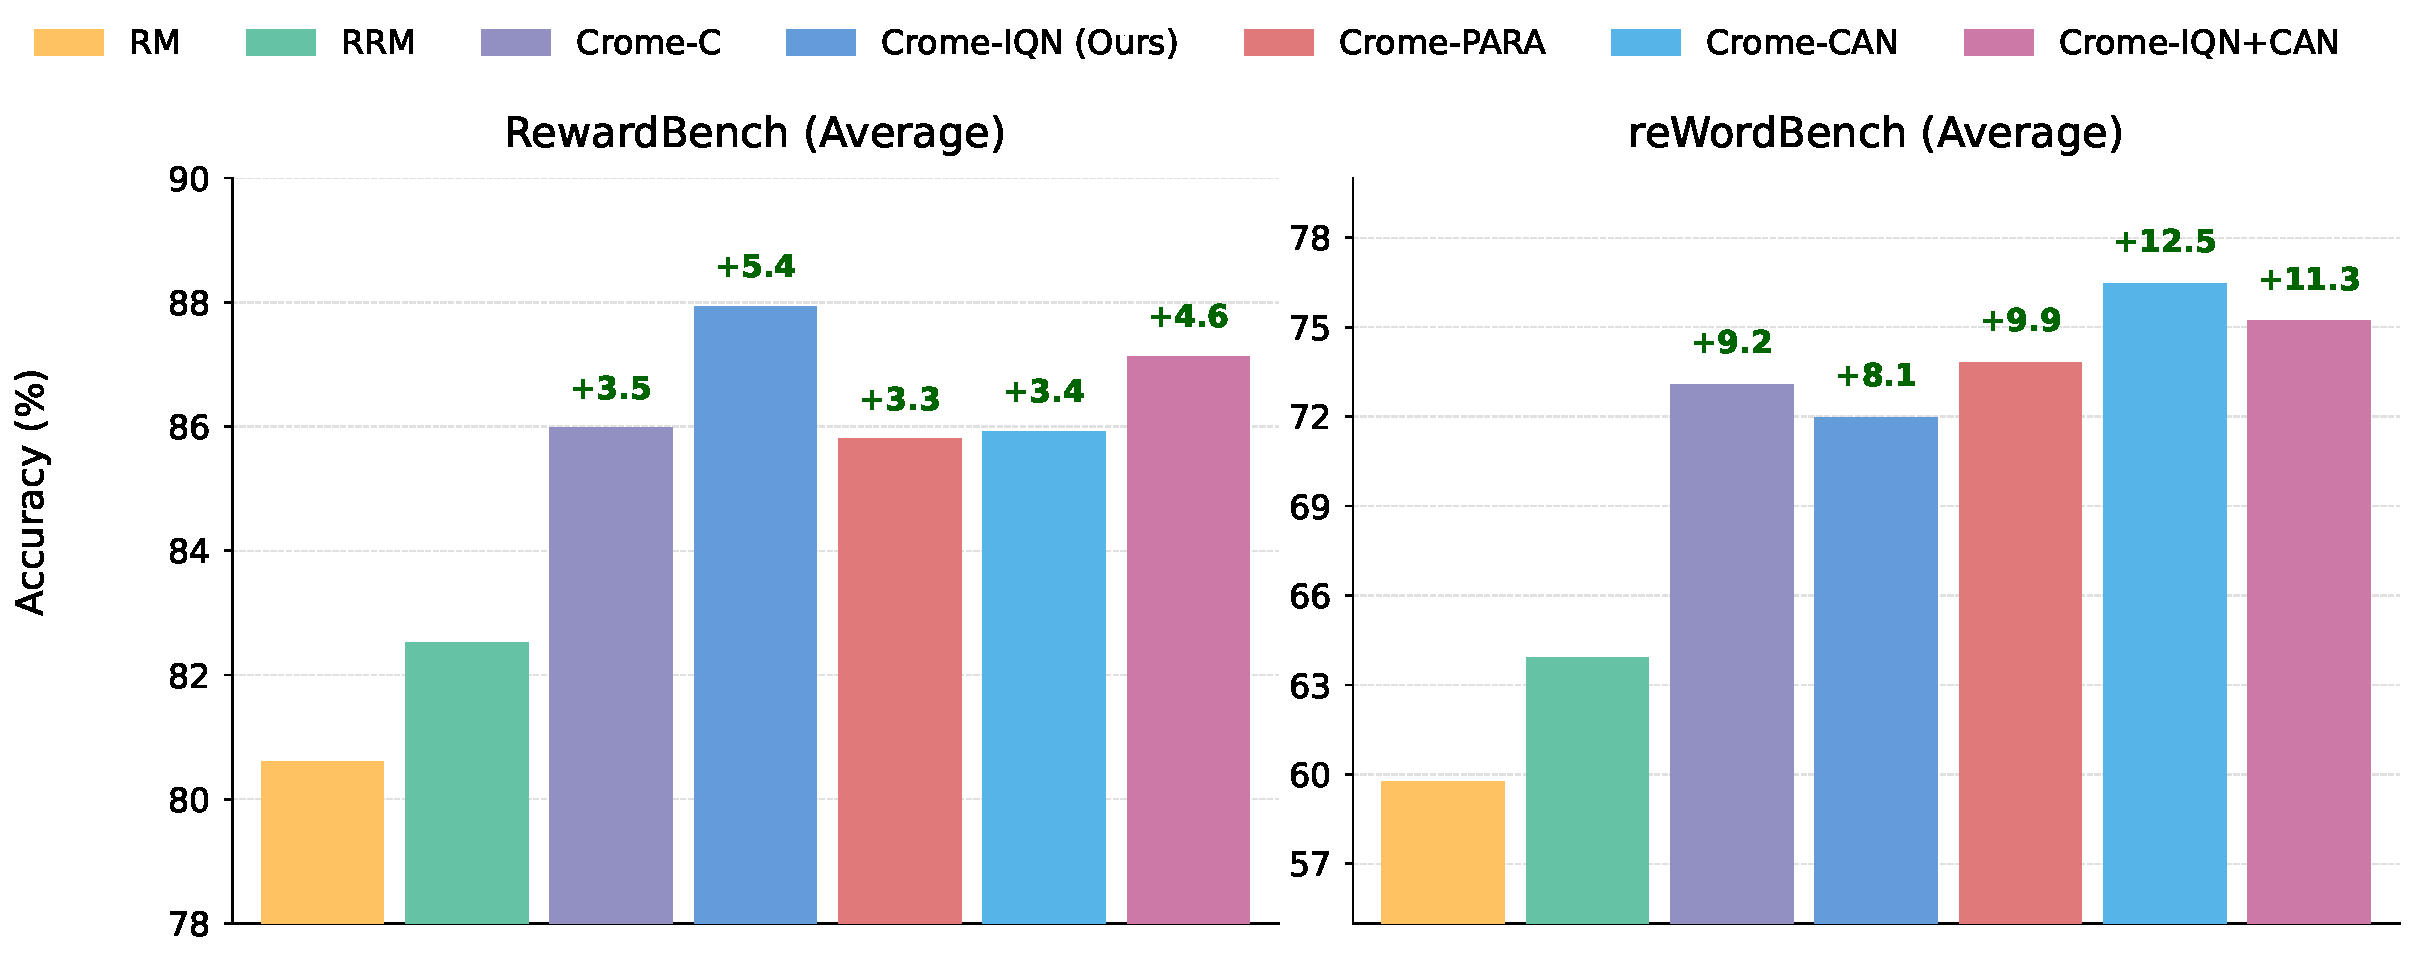
\includegraphics[width=0.95\linewidth]{images/gemma9b_avg_benchmarks_1x2_neutral_augmentations.pdf}
    \vspace{-0.10in}
    \captionof{figure}{Average performance on RewardBench and reWordBench for \carma{} trained with different neutral augmentation strategies. }
    \label{fig:rewordbench-avg_neutral_ablations}
  \end{minipage}

\vspace{0.03in}
\begin{takeawaybox}
\textbf{Key Takeaway:}  \textit{Explicit} suppression of spurious correlates via neutral augmentations mitigates reward hacking by learning \textit{invariant} reward signals, thereby improving downstream performance.
\end{takeawaybox}
\vspace{0.03in}
\end{figure}



\begin{figure}[!ht]
  \centering
  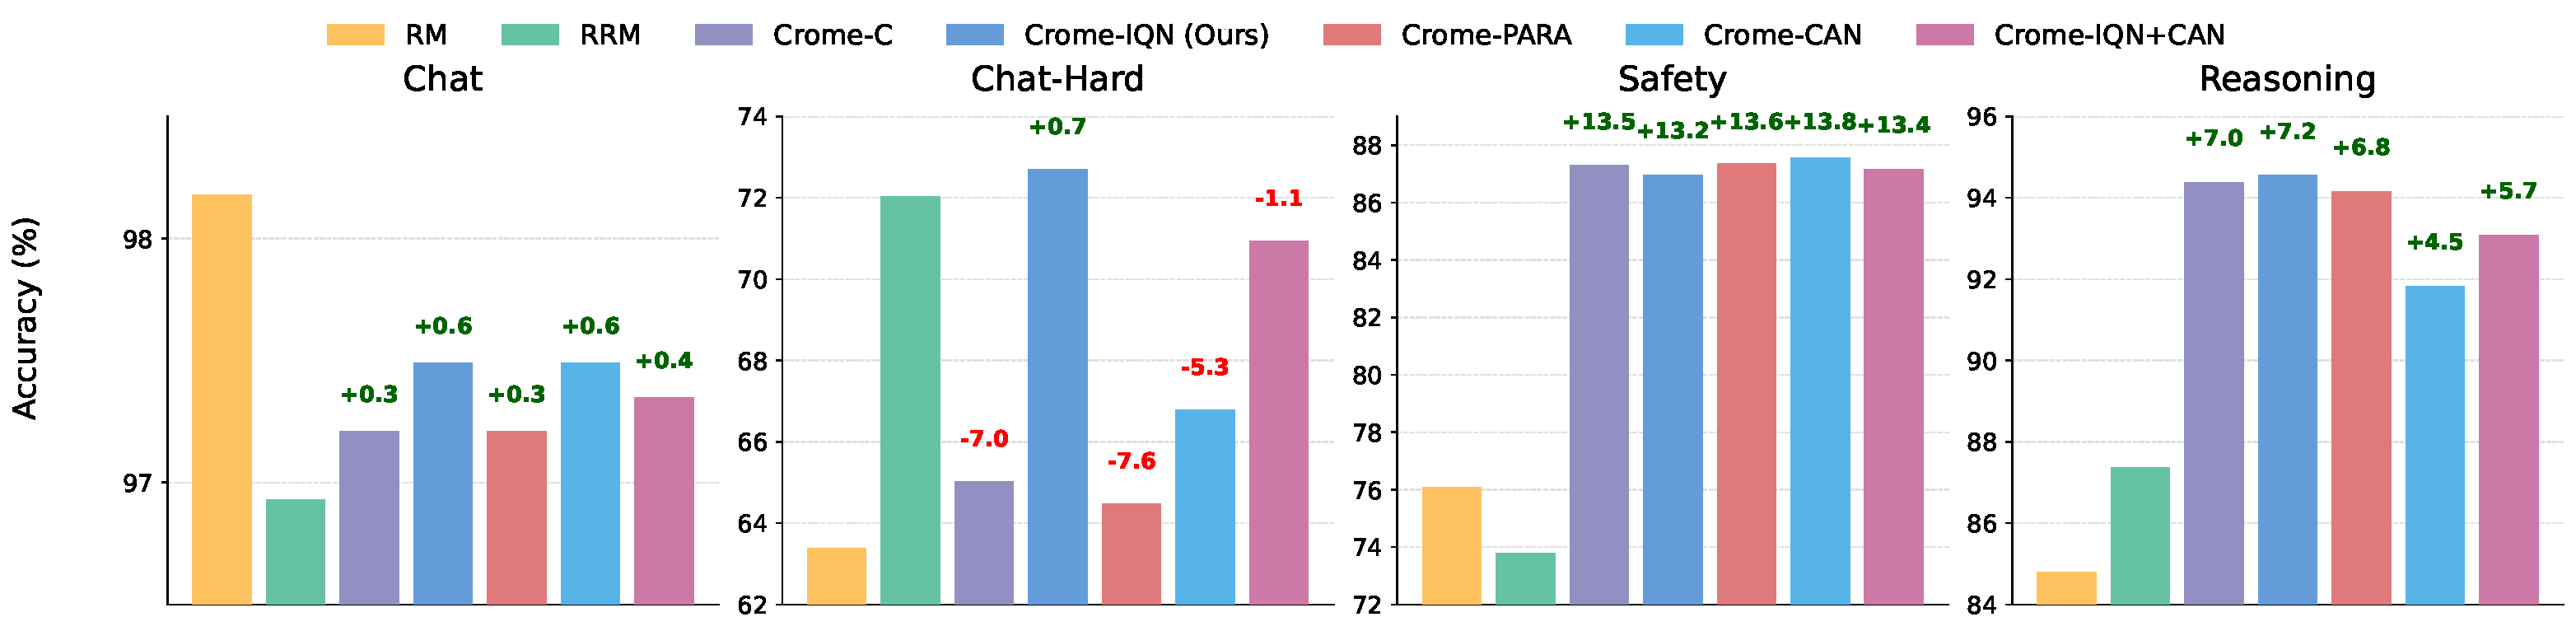
\includegraphics[width=0.95\columnwidth]{images/gemma9b_rewardbench_subsets_1x4_neutral_augmentations.pdf}
  \caption{Evaluations of neutral augmentation variants on the different subsets of RewardBench.}
  \label{fig:rewardbench_subsets_neutral_ablations}
\end{figure}


The \carma{} variants include: \carma{}-C (only causals), \carma{}-IQN (causals + irrelevant query neutrals), \carma{}-PARA
  (causals + paraphrased neutrals), \carma{}-CAN (causals + causally-aligned neutrals), and  \carma{}-IQN+CAN
  (causals + irrelevant query neutrals + 
  causally-aligned neutrals). On the especially challenging \textit{Chat-Hard} subset, \carma{}-IQN performs best. See Appendix Section \ref{sec:causal_model_details} for more details.  Prompts for obtaining these neutrals is given in Appendix \ref{sec:prompt_templates}.
\vspace{0.03in}
\begin{takeawaybox}
\textbf{Key Takeaway:}  A combination of well-designed augmentation strategies, e.g. causal upgradations and degradations, along with IQN produces the most robust and generalizable reward models.
\end{takeawaybox}

\vspace{-0.1in}
\paragraph{Discussion on Neutrals:} 
Our Figure \ref{fig:causal_graph} suggests that interventions along spurious attributes can confound causal attributes in myriad ways. Firstly, there could be causal attributes, which upon intervention can lead to spurious attribute change ($CA\to SP$). Secondly, if spurious attributes change, this can lead to a change in Causal Attributes ($SP\to CA$). Due to such confounding factors, an intervention free solution, such as IQN, turns out to be a clever way to provide invariance to spuriousness.
IQN provides invariance to those spurious factors that change with causal changes (See Fig. \ref{fig:carma_augmentation_visual_overview}), as well as natural spurious variations when irrelevant questions are paired with answers corresponding to a different question.

\vspace{-0.1in}
\paragraph{Ablations and Additional Results:} See Appendix Section \ref{sec:additional_results} where we show that \carma{} exhibits stable and significant improvements in robustness with low variance across different training runs. We also show that using open-weights models as the oracle LLM, such as \gemmathreeit{27}, \carma{} exhibits significant improvements in robustness. Additionally, we also show performance of \carma{} and baselines on in-distribution and out-of-distribution examples, showing superior effective robustness achieved by \carma{}.